\section{Error-prone PCR of a fungal xylanase for improvement of its alkaline and thermal stability}

\subsection{Нормальное название}

Склонная к ошибкам ПЦР (полимеразная цепная реакция) грибковой(очной?) ксиланазы для улучшения её щелочной и термической стабильности.

\subsubsection{Пояснения к вышесказанному}
Ксиланаза -- фермент, расщепляющий полисахарид(ксилан) в моносахарид(ксилоза).

\subsection{Абстракт}
Случайный мутагенез был использован для улучшения щелочной и термической стабильности ксиланазы «название термофильных грибов>>. Были выполнены склонные к ошибка ПЦР; продукты были клонированы в кишечную палочку и библиотека из 960 клонов была отобрана на ксилан-содержащей чашке петри. (ксилан=сахар=еда =>кто умеет его кушать выжил). Полученный грубый фильрат был протестирован (screened) при $80 \mathrm{C}$. При ph 10 Изначальная ксиланаза потеряла 80\% актив-ти после 90 min на 80С и 70\% на ph $10 .$ Наиболее термостабильный же мутант G41 наборот сохранил 75\% активности,а щелочно-стабильный G53 Анализ последовательностей выявил 4 замены аминокислот в G41 и одну в G53. Таким образом эти варианты обладают лучшими термическими/щелочными стабильностями и являются хорошими кандидатами для <<ДНК-шафлингаз>>, чтобы создать в итоге крепкую кслиназу для промышленности.

\subsection{Картинки}
\begin{figure}[H]\label{ul}
	\center{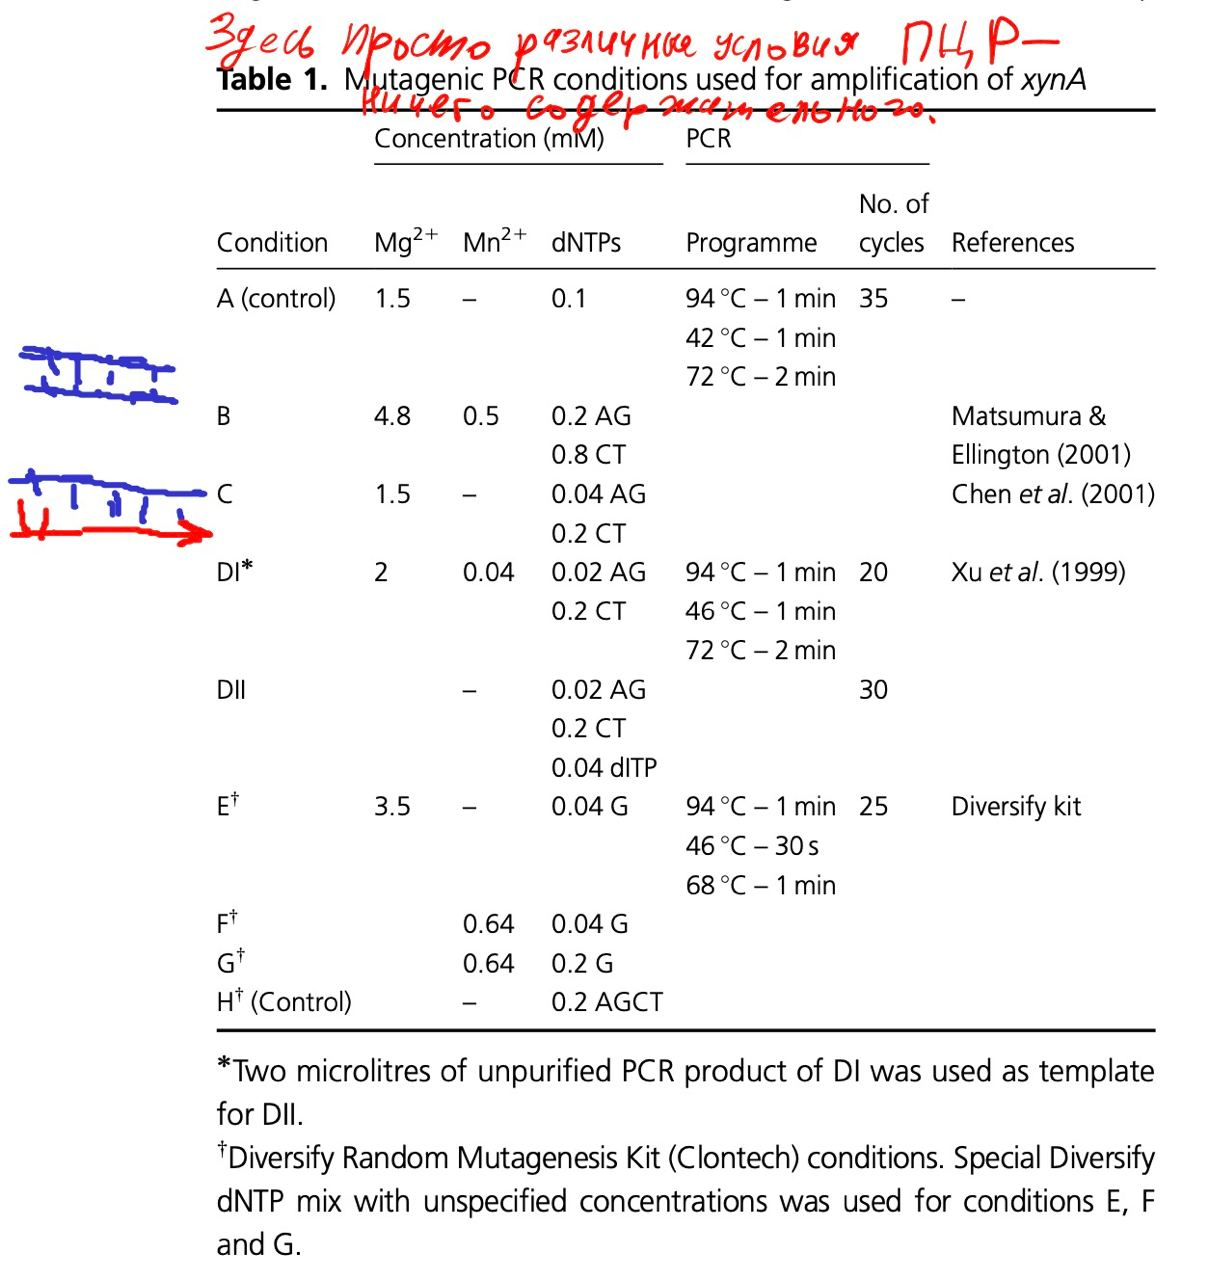
\includegraphics[scale=0.3]{a21.jpg}}
	\caption{Первая картинка}
\end{figure} 

\begin{figure}[H]\label{ul}
	\center{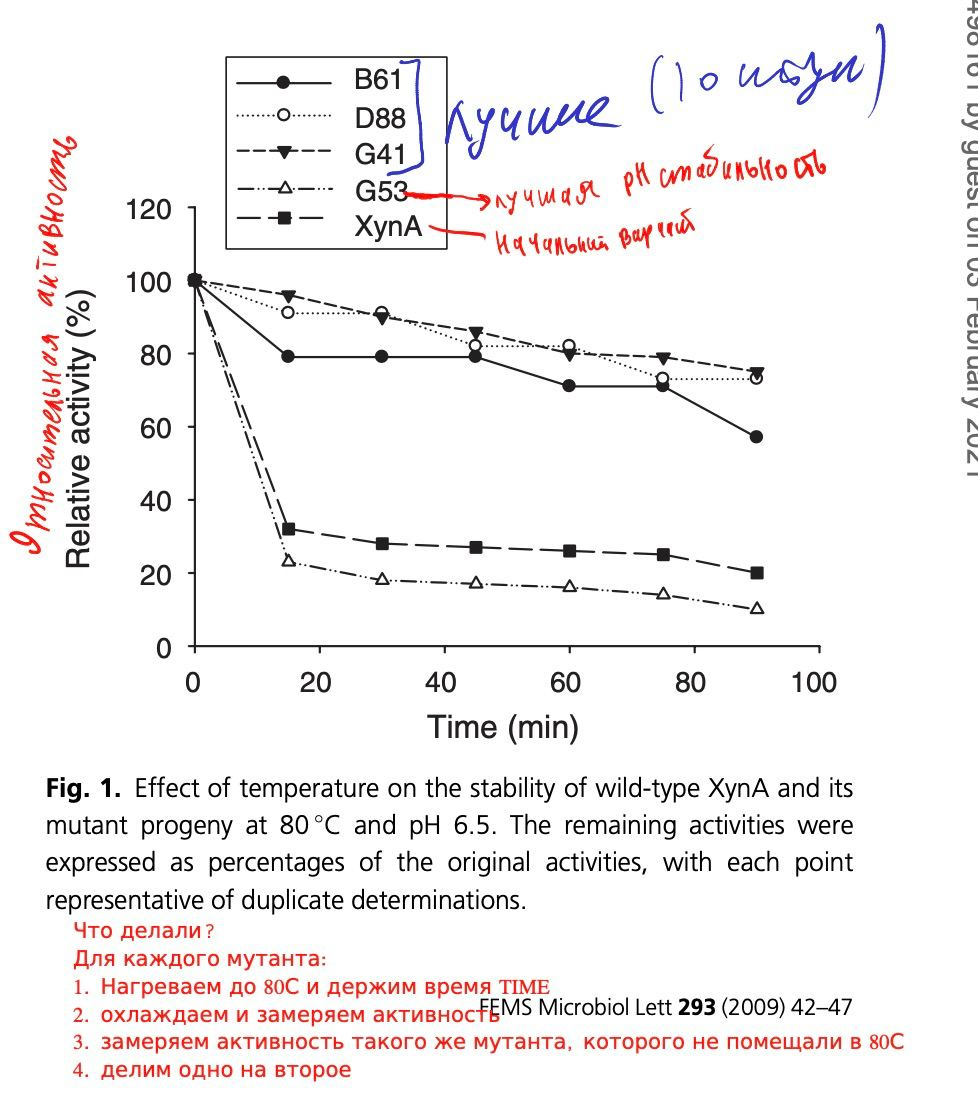
\includegraphics[scale=0.3]{a22.jpg}}
	\caption{Вторая картинка}
\end{figure} 
Видим, что некоторые мутанты теряют сравнительно с диким типом мало активности, кроме того лучший в 10 pH в 80 $^\circ$С теряет еще больше.

\begin{figure}[H]\label{ul}
	\center{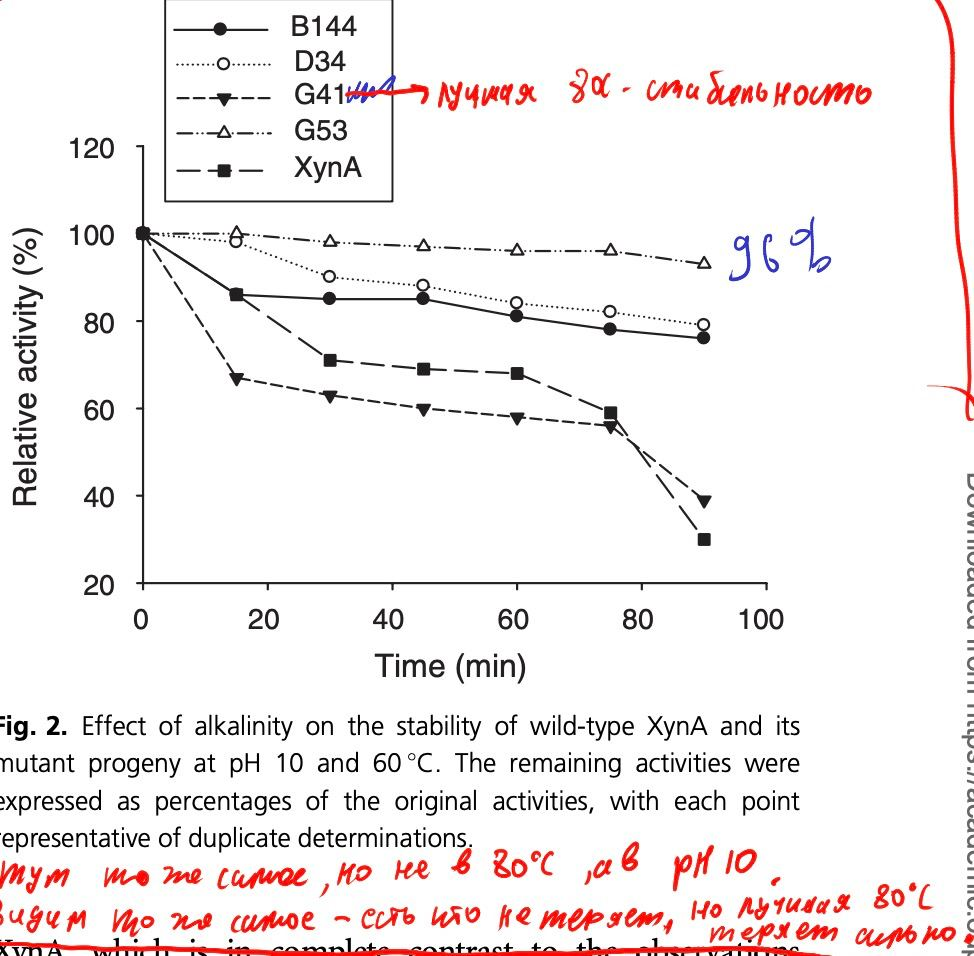
\includegraphics[scale=0.3]{a23.jpg}}
	\caption{Третья картинка}
\end{figure} 


Тут тоже самое, но не в 80 $^\circ$С, а в 10 рН. Видим то же самое -  есть что не теряет, но лучший 80 $^\circ$С теряет сильно.


\begin{figure}[H]\label{ul}
	\center{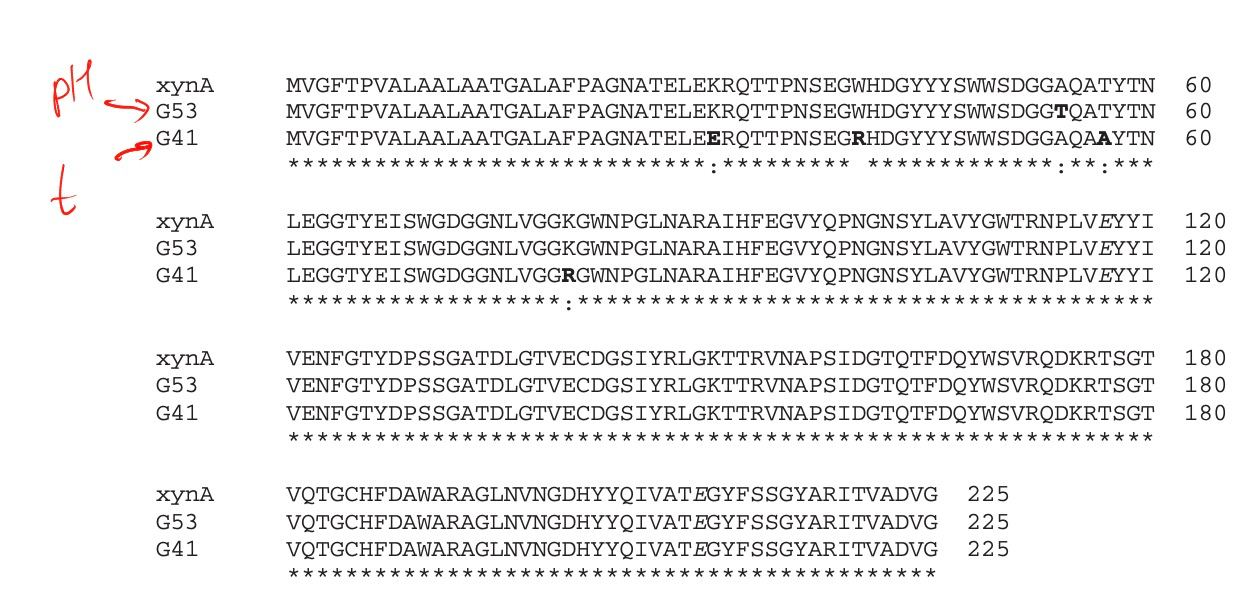
\includegraphics[scale=0.3]{a24.jpg}}
	\caption{Четвертая картинка}
\end{figure} 
Сравнение последовательностей аминокислот оригинальной ксилианзы и лучшей по 80 $^\circ$С и лучшей по 10 рН стабильности.